\subsection{New Zealand model v2 (model ID: 16)}
The New Zealand model v2 (fig.~\ref{fig:16_schematic}) is part of a top-down modelling exercise (referred to as "Model A") that focusses on several catchments in New Zealand \citep{Atkinson2003}. It has 2 stores and 8 parameters ($I_{max}$, $S_{max}$, $S_{fc}$, $M$, $a$, $b$, $t_{c,bf}$ and $d$). The model aims to represent:

\begin{itemizecompact}
\item Interception by vegetation;
\item Separate vegetation and bare soil evaporation;
\item Saturation excess overland flow;
\item Subsurface runoff when soil moisture exceeds field capacity;
\item Baseflow;
\item Flow routing.
\end{itemizecompact}

\subsubsection{File names}
\begin{tabular}{@{}ll}
Model: &m\_16\_newzealand2\_8p\_2s \\
Parameter ranges: &m\_16\_newzealand2\_8p\_2s\_parameter\_ ranges \\
\end{tabular}

% Equations
\subsubsection{Model equations}

% Model layout figure
{ 																	% This ensures it doesn't warp text further down
\begin{wrapfigure}{l}{6.5cm}
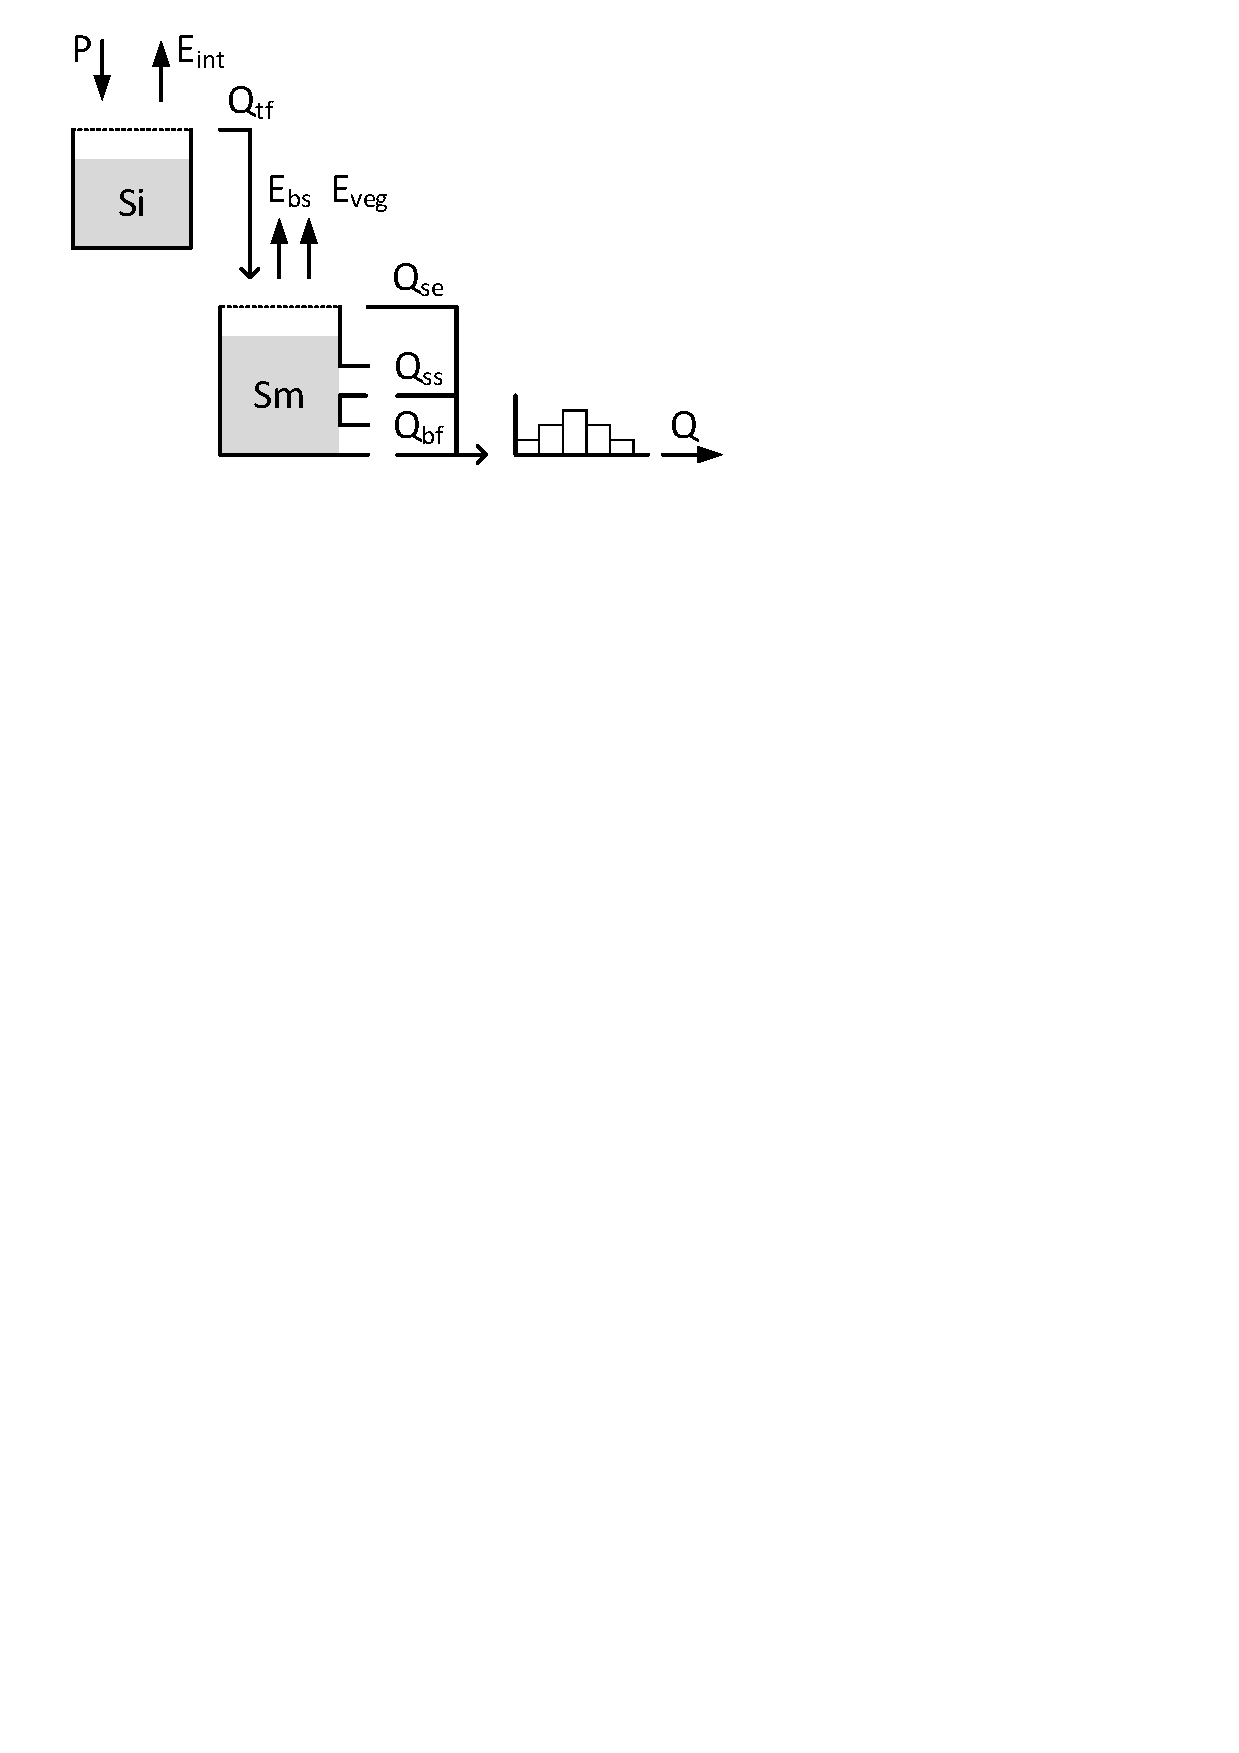
\includegraphics[trim=1cm 22cm 7cm 1cm,width=7cm,keepaspectratio]{./files/16_schematic.pdf}
\caption{Structure of the New Zealand model v1} \label{fig:16_schematic}
\end{wrapfigure}

\begin{align}
	\frac{dS_i}{dt} &= P - E_{int} - Q_{tf}\\
	E_{int} &= Ep \\
	Q_{tf} &= \begin{cases}
		P, &\text{if } S_i \geq I_{max}\\
		0, &\text{otherwise}\\
	\end{cases}
\end{align}

Where  $S_i$ [mm] is the current interception storage which gets replenished through daily precipitation $P$ $[mm/d]$. Intercepted water is assumed to evaporate ($E_{int}$ $[mm/d]$) at the potential rate $E_p$ $[mm/d]$ when possible. $Q_{tf}$ $[mm/d]$ represents throughfall towards soil moisture when the interception store is at maximum capacity $I_{max}$ [mm].

} % end of wrapfigure fix

\begin{align}
	\frac{dS_m}{dt} &= Q_{tf} - E_{veg} - E_{bs}  - Q_{se} - Q_{ss} - Q_{bf}\\
	E_{veg} &= \begin{cases}
		M*E_p, &\text{if } S > S_{fc} \\
		\frac{S_m}{S_{fc}}*M*E_p, &\text{otherwise} \\
	\end{cases} \\
	E_{bs} &= \frac{S}{S_{max}}(1-M)*E_p \\
	Q_{se} &= \begin{cases}
		P, &\text{if } S \geq S_{max}\\
		0, &\text{otherwise}\\
	\end{cases}\\
	Q_{ss} &= \begin{cases}
		\left(a*(S-S_{fc})\right)^b, &\text{if } S \geq S_{fc} \\
		0, &\text{otherwise}\\
		\end{cases}\\
	Q_{bf} &= t_{c,bf}*S	
\end{align}

Where $S_m$ [mm] is the current soil moisture storage which gets replenished through daily precipitation $P$ $[mm/d]$. Evaporation through vegetation $E_{veg}$ $[mm/d]$ depends on the forest fraction $M$ [-] and field capacity $S_{fc}$ [-]. $E_{bs}$ $[mm/d]$ represents bare soil evaporation. When S exceeds the maximum storage $S_{max}$ [mm], water leaves the model as saturation excess runoff $Q_{se}$. If S exceeds field capacity $S_{fc}$ [mm], subsurface runoff $Q_{ss}$ $[mm/d]$ is generated controlled by time parameter $a$ $[d^{-1}]$ and nonlinearity parameter $b$ [-]. $Q_{bf}$ represents baseflow controlled by time scale parameter $t_{c,bf}$ $[d^{-1}]$. Total runoff $Q_t$ $[mm/d]$ is:

\begin{equation}
	Q_t = Q_{se} + Q_{ss} + Q_{bf}
\end{equation}

Total flow is delayed by a triangular routing scheme controlled by time parameter $d$ [d].

\subsubsection{Parameter overview}
% Table generated by Excel2LaTeX from sheet 'Sheet1'
\begin{table}[htbp]
  \centering
    \begin{tabular}{lll}
    \toprule
    Parameter & Unit  & Description \\
    \midrule
    $I_{max}$ & $mm$  & Maximum interception capacity \\
    $S_{max}$ & $mm$  & Maximum soil moisture storage \\
    $S_{fc}$ & $mm$  & Field capacity \\
    $M$   & $-$   & Forest fraction \\
    $a$   & $d^{-1}$ & Runoff coefficient \\
    $b$   & $-$   & Runoff nonlinearity \\
    $t_{c,bf}$ & $d^{-1}$ & Runoff coefficient \\
    $d$   & $d$   & Unit Hydrograph time base \\
    \bottomrule
    \end{tabular}%
  \label{tab:addlabel}%
\end{table}%

